\documentclass[algorithmlist, figurelist,tablelist, nomlist,engineering]{seuthesix}


\begin{document}
\categorynumber{000} % 分类采用《中国图书资料分类法》
\UDC{000}            %《国际十进分类法UDC》的类号
\secretlevel{公开}    %学位论文密级分为"公开"、"内部"、"秘密"和"机密"四种
\studentid{130623}   %学号要完整,前面的零不能省略。
\title{灵犀一指心法}{灵犀一指}{The theory of powerful fingers}{powerful fingers}
\author{陆小凤}{Phoenix Land, Jr.}
\advisor{夜帝}{教授}{King Night}{Prof.}
\coadvisor{楚留香}{副教授}{Perfume Tsu}{Associate Prof.} % 没有% 可以不填
 \degreetype{武学硕士}{Master of kung fu} % 详细学位名称
\major{内功}
\submajor{内功心法}
\defenddate{\today}
\authorizedate{\today}
\committeechair{夜帝}
\reviewer{张三丰}{黄药师}
\department{东南大学武学院}{School of kung fu}
\seuthesisthanks{本课题的研究获郭靖-黄蓉降龙基金、杨过-小龙女黯然销魂基金以及郭襄的倚天基金资助}
\makebigcover
\makecover
\begin{abstract}{武功,心法,内功,灵犀一指}
灵犀一指是一种非常厉害的武功。
\end{abstract}

\begin{englishabstract}{kung fu, theory, fundamental kung fu, powerful fingers}
 powerful fingers is a kind of powerful kung fu.
\end{englishabstract}

\setnomname{术语与符号约定}
\tableofcontents
\listofothers

\mainmatter

\chapter{绪论}
\section{研究背景}
天下武功,无坚不破,唯快不破。灵犀一指属于快而非坚之武学。


\section{本论文的工作}
本论文的研究对象为灵犀一指,着重研究其中的内功心法。


\nomenclature{PF}{powerful fingers}
\nomenclature{KF}{kung fu}

\chapter{武学与江湖}

\section{引言}
行走江湖义当先,路见不平,拔刀相助。

\section{人与江湖}
有人的地方就有江湖,江湖险恶。

\section{武学的博大精深}
天下武学,博大精深。若心生贪念,修行邪术,终将走火入魔。

\section{本章小结}
本章介绍了武学,江湖与人的关系。为后续章节的内容打下了基础。

\chapter{内功}
\section{引言}
内功是指提升人内力的武功,与招式相对。内功是招式的理论,招式是内功的技术。

\section{内功的基本原理}
气聚丹田,心无杂念方可修行内功。

\section{内功与喝酒的关系}
研究表明,适量饮酒有助于修炼内功。



\section{本章小结}
本章主要介绍了内功的基本概念、原理。

\chapter{心法}
\section{引言}
内功即是武学的理论,而心法就是内功的核心部分。
\section{如何提高内功}
提高内功只有勤加修炼,尤其是心法的修炼。
\section{本章小结}
本章介绍了心法和内功的关系。

\chapter{灵犀一指}
\section{引言}
灵犀一指是陆小凤自创的一门武功。这种武功不需要任何兵器,只需徒手就可将敌人制服。

\section{灵犀一指的起源}
陆小凤年轻时热衷武学,在西域一代游历时突发灵感,创立了灵犀一指,如图\ref{lxfbook}所示。

\begin{figure}
\centering
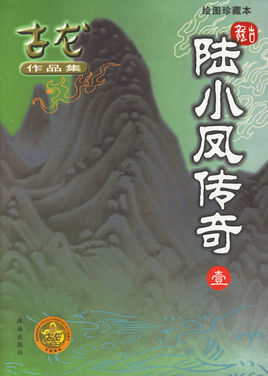
\includegraphics[width=.6\textwidth]{lxfbook.jpg}
\caption{陆小凤传奇\label{lxfbook}}
\end{figure}

\section{灵犀一指要诀}
灵犀一指是一种以柔制刚的武功,一般人很难领悟其中的精妙之处,因此很难学会。\cite{lxf:a}\citen{lxf:b}
实际上,它的要诀就是将内力汇聚在手指经脉之内,提高内力的密度,然后在瞬间释放出来,以致达到将敌人兵器折断的力道。
如表\ref{lxfinsight}所示。
\begin{table}
\centering
\caption{灵犀一指的要诀\label{lxfinsight}}
\begin{tabular}{|c||c|}
\hline
步骤 & 操作\\
\hline\hline
1 &  气聚丹田\\
\hline
2 & 将丹田之气注入手指经脉\\
\hline
3 & 瞬间释放\\
\hline
4 & 将敌人制服\\
\hline
\end{tabular}
\end{table}

也可用算法表示,如算法\ref{algoinsight}所示。

\begin{algorithm}
\caption{\label{algoinsight}灵犀一指要诀}
\begin{algorithmic}[1]
\STATE 气聚丹田。
\STATE 将丹田之气注入手指经脉。
\STATE 瞬间释放。
\STATE 将敌人制服。
\end{algorithmic}
\end{algorithm}

也可用数学公式表示,如式\ref{mc2}所示。
\begin{equation}
E=mc^2
\label{mc2}
\end{equation}

\section{本章小结}
本章介绍了灵犀一指的要诀部分。




\chapter{全文总结}
本文介绍了灵犀一指的起源,重要性和其中的要诀。
本章对全文工作进行了回顾和总结。

\acknowledgement
感谢每一个给予帮助的人。

\thesisbib{seuthesix}


\appendix

\chapter{欧几里得第二定理的证明}
\newtheorem{theorem}{定理}
\begin{theorem}
欧几里得第二定理(素数有无穷多个)\\
证明:用反证法。假设素数有有限个($N$个),记为$p_1,p_2,\dots,p_N$。则我们构造一个新的数,
\[
n=p_1p_2\dots p_N+1.
\]
由于$p_i,i=1,2,\dots,N$为素数,则一定不为$1$。于是对于任意的$p_i,i=1,2,\dots, N$,有
\[
p_i\not|n
\]
这表明,要么$n$本身为素数,要么$n$为合数,但是存在$p_1,p_2,\dots,p_N$之外的其他素数能够将$n$进行素因子分解。
不管哪种情况,都表明存在更多的素数。定理得证。\qed
\end{theorem}

\chapter{$\sqrt{2}$是无理数的证明}
\begin{theorem}
$\sqrt{2}$是无理数。\\
证明:用反证法。假设$\sqrt{2}$是有理数,则可表示为两个整数的商,即$\exists p,q, q\ne0$
\[
\sqrt{2}=\frac{p}{q}
\]
不失一般性,我们假设$p,q$是既约的,即$\gcd(p,q)=1$。对上式两边平方可得\\
\begin{align*}
2& =\frac{p^2}{q^2}\\
p^2&=2q^2.
\end{align*}
表明$p^2$为偶数,因此$p$为偶数,记$p=2m$。则
\begin{align*}
p^2&=4m^2=2q^2\\
q^2&=2m^2.
\end{align*}
表明$q$也为偶数,因此它们有公共因子$2$。这与它们既约的假设矛盾。定理得证。\qed
\end{theorem}

\resume{作者攻读硕士学位期间的研究成果}
\begin{flushleft}
{\bfseries \large 发表的论文}\\ \relax
[1] 第一作者,“灵犀一指:理论与应用”, 武侠学报,
2015年5月。\\
\end{flushleft}


\end{document}